\section{Results}
\label{sec:results}

\subsection{Training Performance}
\label{sec:training}

\Tabref{tab:training} summarizes validation loss for each model relative to the maximum-entropy baseline. The \rpscounter model achieves the lowest loss (0.554), reflecting the high predictability of the counter strategy. \rpsrandom reaches the entropy ceiling (1.099), confirming no learnable pattern exists. \messthree with $p=0.6$ barely learns (loss 1.091 vs.\ entropy 1.099), indicating the weak emission signal is nearly indistinguishable from random.

\begin{table}[t]
\caption{Training performance across datasets. The learning signal column shows the gap between validation loss and the maximum-entropy baseline $\log |\mathcal{V}|$.}
\label{tab:training}
\centering
\begin{tabular}{@{}lccc@{}}
\toprule
Dataset & Best Val Loss & Entropy Baseline & Learning Signal \\
\midrule
\messthree ($p{=}0.9$) & 0.925 & 1.099 & 0.174 \\
\messthree ($p{=}0.6$) & 1.091 & 1.099 & 0.008 \\
\rpscounter & {\bf 0.554} & 1.099 & {\bf 0.546} \\
\rpsrandom & 1.099 & 1.099 & 0.000 \\
\rpswsls & 0.918 & 1.099 & 0.181 \\
\ttt & 1.271 & 2.197 & 0.926 \\
\bottomrule
\end{tabular}
\end{table}

\subsection{Participation Ratio Across Context Positions}
\label{sec:pr_results}

\para{Stationary processes show flat geometry.}
\Figref{fig:pr_vs_pos} shows participation ratio as a function of context position. For stationary processes (\messthree and RPS), $\PR$ stabilizes within the first ${\sim}5$ positions and remains approximately constant thereafter. \messthree ($p=0.9$) shows no significant trend ($\rho = -0.079$, $p = 0.69$), with $\PR$ hovering around 2.0--2.4 throughout the context window. \rpscounter ($\rho = 0.069$, $p = 0.73$) and \rpswsls ($\rho = 0.028$, $p = 0.89$) are similarly flat.

\para{\ttt shows dramatic collapse.}
In contrast, \ttt exhibits a striking dimensionality collapse from $\PR = 7.85$ at position 0 to $\PR = 1.26$ at the final position. This represents a near-total geometric simplification, with Cohen's $d = 19.98$ between early and late positions (\tabref{tab:early_late}). The collapse directly mirrors the shrinking number of legal moves: at position 0, all 9 board cells are available; by the final move, only one remains.

\begin{figure}[t]
\centering
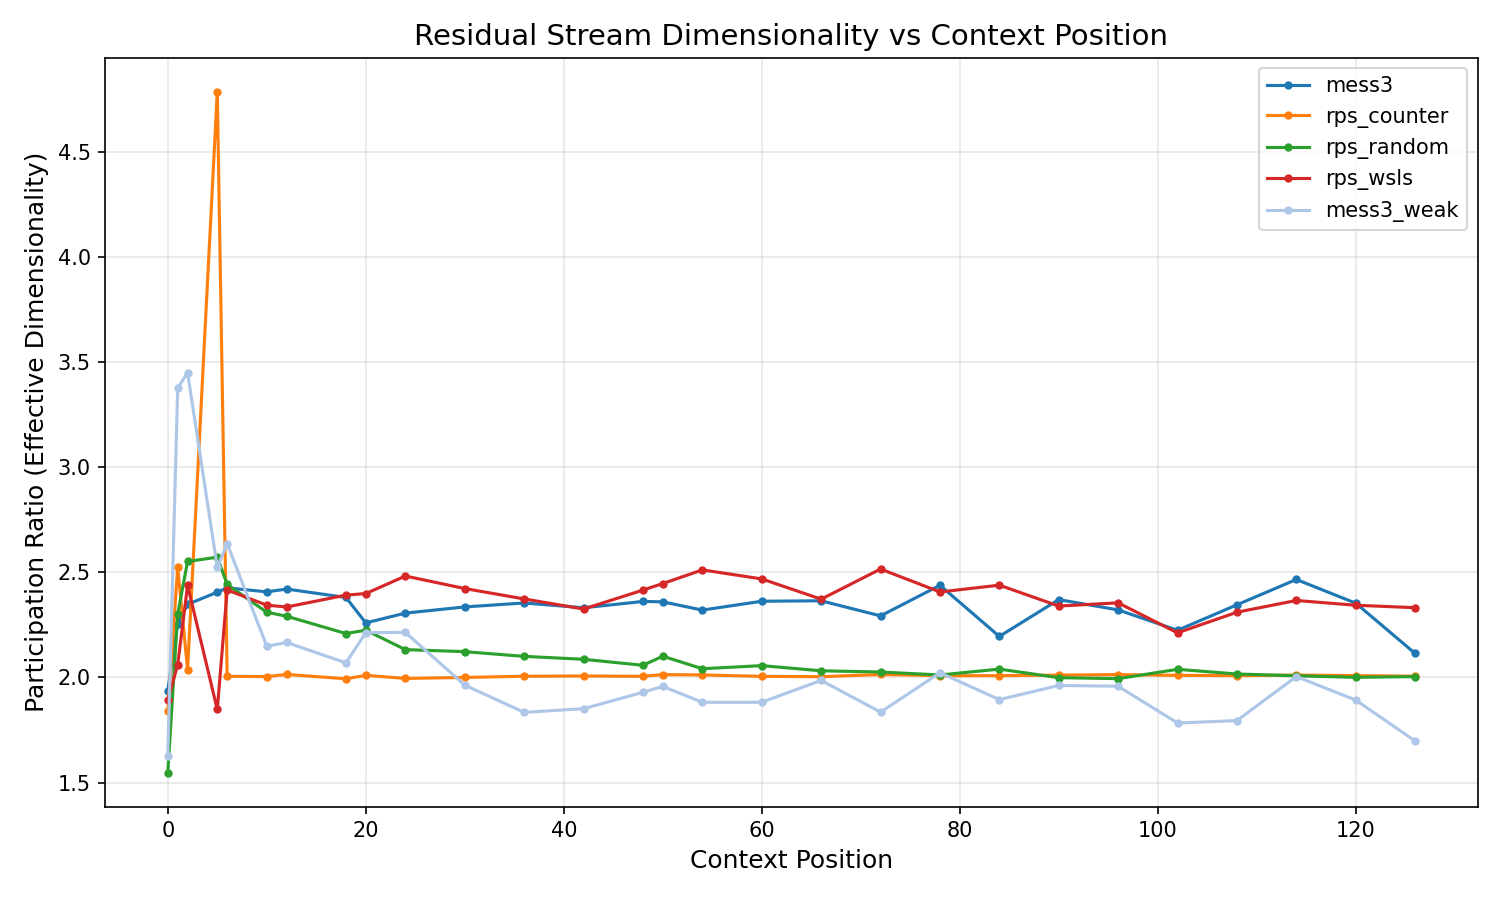
\includegraphics[width=0.95\linewidth]{../results/plots/participation_ratio_vs_position.png}
\caption{Participation ratio vs.\ context position for all datasets. Stationary processes (\messthree, RPS variants) maintain approximately constant $\PR \approx 2.0$--$2.3$ across the full context window. \ttt shows dramatic dimensionality collapse ($\PR$: $7.85 \to 1.26$) as the game board fills and fewer legal moves remain.}
\label{fig:pr_vs_pos}
\end{figure}

\begin{table}[t]
\caption{Early vs.\ late context position comparison. Early = positions 0--9, late = positions 118--127 (or final positions for \ttt). Cohen's $d$ and $t$-test $p$-values assess the magnitude and significance of the difference.}
\label{tab:early_late}
\centering
\begin{tabular}{@{}lcccc@{}}
\toprule
Dataset & Early $\PR$ & Late $\PR$ & Cohen's $d$ & $p$-value \\
\midrule
\messthree ($p{=}0.9$) & 2.31 & 2.31 & 0.005 & 0.993 \\
\messthree ($p{=}0.6$) & 2.56 & 1.87 & 1.562 & 0.019 \\
\rpscounter & 2.46 & 2.01 & 0.653 & 0.280 \\
\rpsrandom & 2.29 & 2.01 & 1.228 & 0.055 \\
\rpswsls & 2.31 & 2.33 & --- & --- \\
\ttt & 8.17 & 1.60 & {\bf 19.98} & {\bf 0.005} \\
\bottomrule
\end{tabular}
\end{table}

\para{The $\PR \approx 2$ floor.}
All models with a 3-token vocabulary converge to $\PR \approx 2.0$ at late positions, regardless of the data-generating process or whether the model has learned anything (\eg \rpsrandom achieves $\PR \approx 2.0$ despite learning no structure). This is consistent with the simplex structure of 3-token distributions: the model maps inputs into a 2-dimensional belief simplex, yielding $\PR \approx 2$.

\subsection{Belief State Regression}
\label{sec:belief}

For \messthree, we regress residual stream activations onto ground-truth Bayesian belief state vectors using ridge regression. \Figref{fig:belief} shows $R^2$ as a function of context position.

\para{Regression quality decreases with context.}
Contrary to the hypothesis that more context should improve internal representations, $R^2$ \emph{decreases} across context positions for both emission strengths. For $p = 0.9$, $R^2$ drops from 1.000 at position 0 to 0.952 at position 126 (Spearman $\rho = -0.782$, $p < 0.001$). For $p = 0.6$, the degradation is more pronounced: $R^2$ drops from 1.000 to 0.835 ($\rho = -0.900$, $p < 0.001$). This suggests that the model's residual stream representation drifts from optimal belief states at later positions.

\begin{figure}[t]
\centering
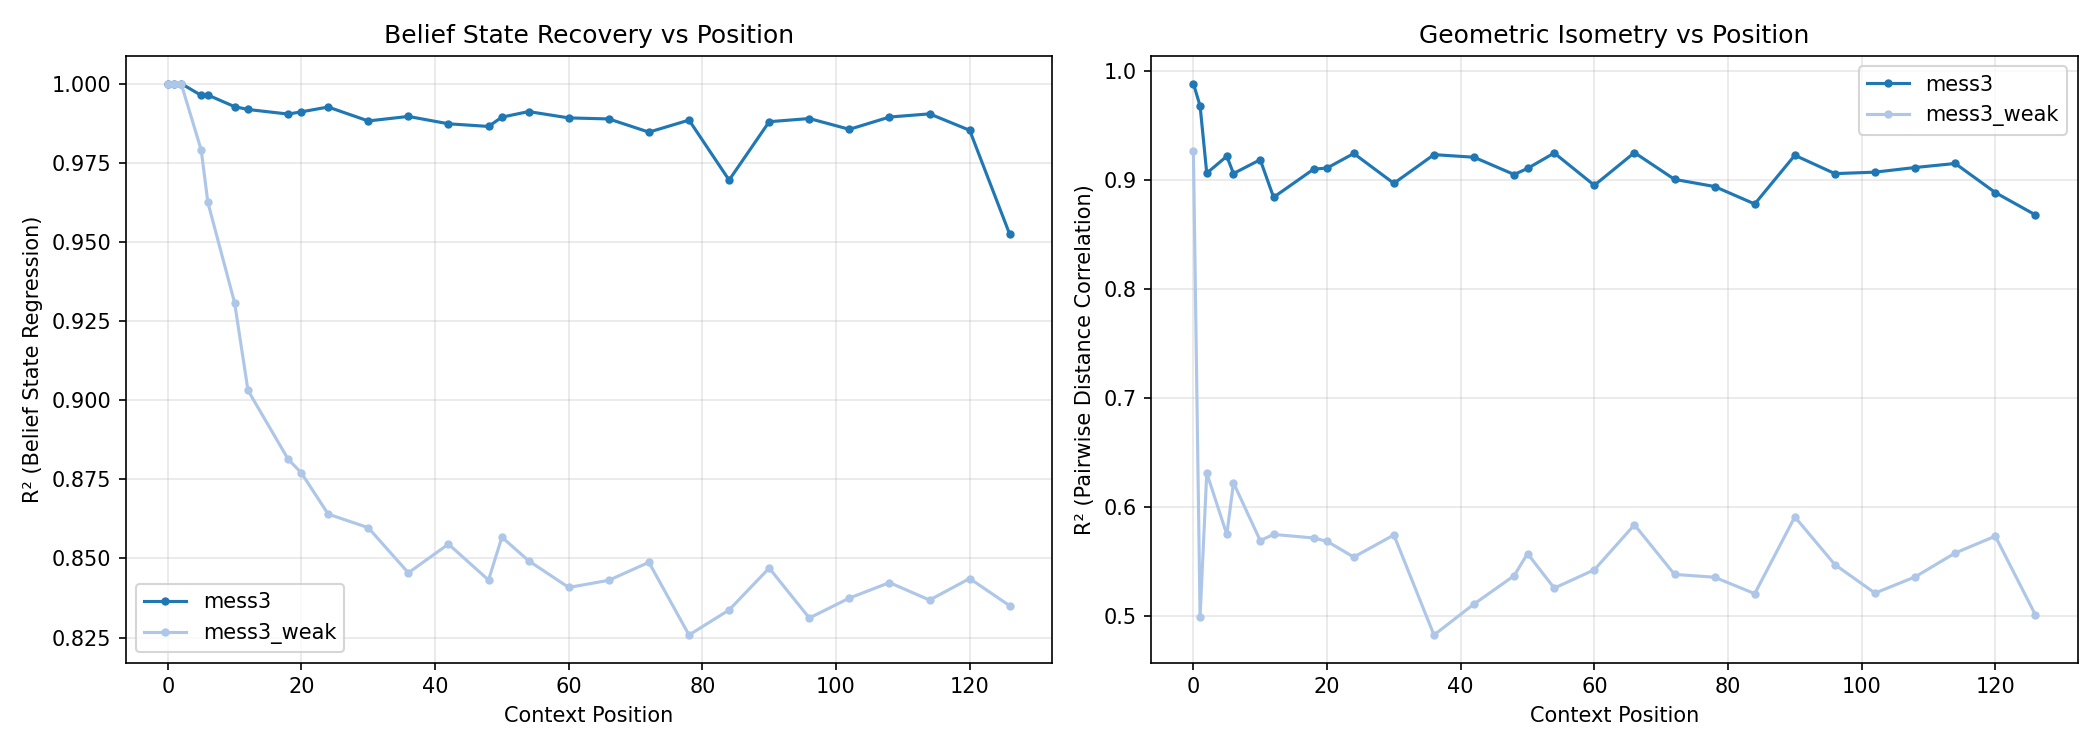
\includegraphics[width=0.95\linewidth]{../results/plots/belief_state_regression.png}
\caption{Belief state regression $R^2$ vs.\ context position for \messthree. Despite the model seeing more context at later positions, regression quality \emph{decreases}, dropping from $R^2 = 1.0$ to $0.95$ ($p = 0.9$) and $0.84$ ($p = 0.6$). This indicates representational drift rather than progressive refinement.}
\label{fig:belief}
\end{figure}

\subsection{Hypothesis Testing Summary}
\label{sec:hypothesis_summary}

\Tabref{tab:hypotheses} summarizes the outcome of each pre-registered hypothesis.

\begin{table}[t]
\caption{Pre-registered hypothesis outcomes. We evaluate each hypothesis against the experimental evidence, reporting the key statistical test and our assessment.}
\label{tab:hypotheses}
\centering
\resizebox{\textwidth}{!}{
\begin{tabular}{@{}p{0.40\textwidth}lp{0.35\textwidth}@{}}
\toprule
Hypothesis & Outcome & Evidence \\
\midrule
H1: $\PR$ decreases with context position & Partially supported & True for \ttt ($d = 19.98$) and \messthree-weak ($p = 0.002$), but not for \messthree-strong or \rpscounter \\
H2: Probe accuracy increases with position & Not supported & Approximately flat or decreasing across positions \\
H3: Structured strategies $\to$ faster simplification & Not supported & \rpsrandom shows strongest $\PR$ decrease ($\rho = -0.749$); structured strategies are flat \\
H4: Simpler games $\to$ lower dimensionality & Supported & \ttt starts at $\PR = 7.85$ (10-token vocab); all 3-token games at $\PR \approx 2$ \\
\bottomrule
\end{tabular}
}
\end{table}

\subsection{Layer-wise Analysis}
\label{sec:layers}

We compute $\PR$ at each layer to understand where geometric structure emerges. Across all datasets, later layers show lower participation ratios than earlier layers, consistent with progressive compression through the network. The final layer consistently produces the most geometrically simple representations. However, the \emph{trend across context positions} is consistent across layers: stationary-process geometry remains flat at every layer, while \ttt collapses at every layer.

\subsection{Random Model Comparison}
\label{sec:random_baseline}

Random (untrained) models produce $\PR$ values similar to trained models for \messthree (random: $1.94 \to 2.05$; trained: $1.94 \to 2.11$). This indicates that the $\PR \approx 2$ floor is partly an architectural property of the 64-dimensional model with 3-token vocabulary, not solely a consequence of learning. The trained model's geometry is shaped more by architectural constraints than by learned structure at this scale.
